\section{Mesures et identification}

\subsection{EX1 — Paramètres électriques \texorpdfstring{\(R\)}{R} et \texorpdfstring{\(L\)}{L}}

\subsubsection{Protocole}

Un échelon de tension est appliqué à la bobine. Deux essais sont réalisés :
\begin{itemize}
    \item \textbf{Essai avec mouvement} (\texttt{T0000ALL.CSV}) : l'actionneur est libre de se déplacer ;
    \item \textbf{Essai maintenu} (\texttt{T0001ALL.CSV}) : l'actionneur est maintenu immobile (\(\dot{\alpha}=0\)).
\end{itemize}

La voie CH1 mesure la tension \(u\) aux bornes de la bobine, CH2 mesure le courant via la sonde (\(\SI{1}{A/V}\)). L'essai maintenu est théoriquement nécessaire pour éliminer la f.c.e.m. et obtenir \(R\) et \(L\) directement. L'essai avec mouvement permet d'observer l'influence de la f.c.e.m.\ sur la réponse transitoire.

\subsubsection{Signaux bruts}

\begin{figure}[H]
\centering
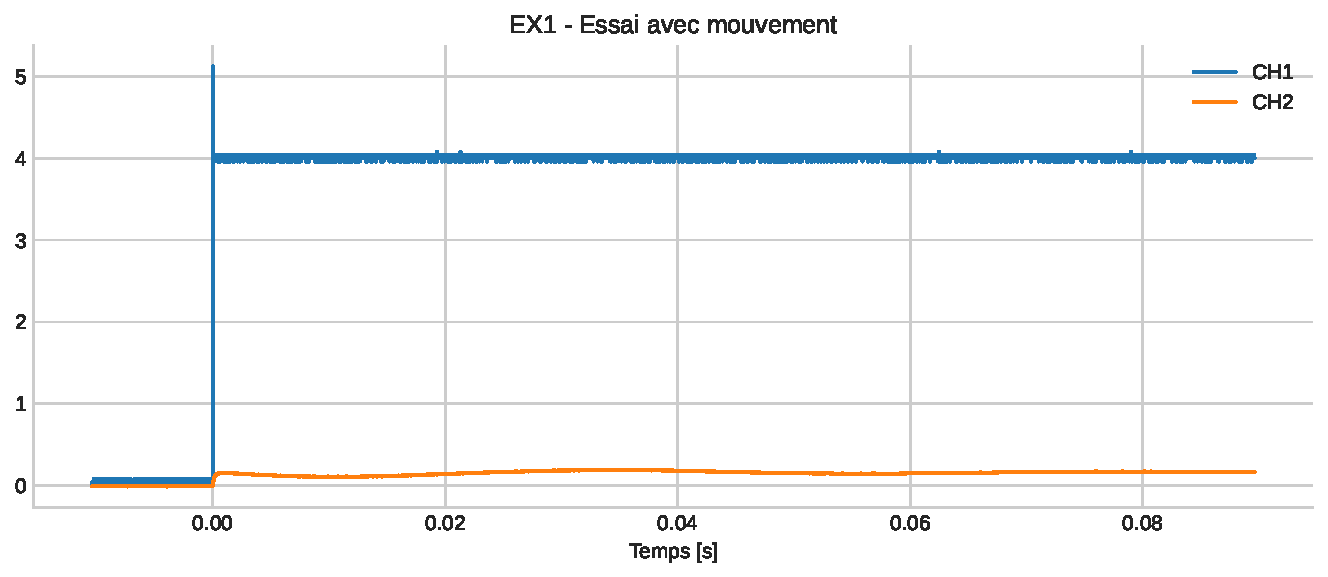
\includegraphics[width=0.9\textwidth]{images/fig_ex1_moving.pdf}
\caption{EX1 — Tension et courant lors de l'essai avec mouvement}
\label{fig:ex1_moving}
\end{figure}

\begin{figure}[H]
\centering
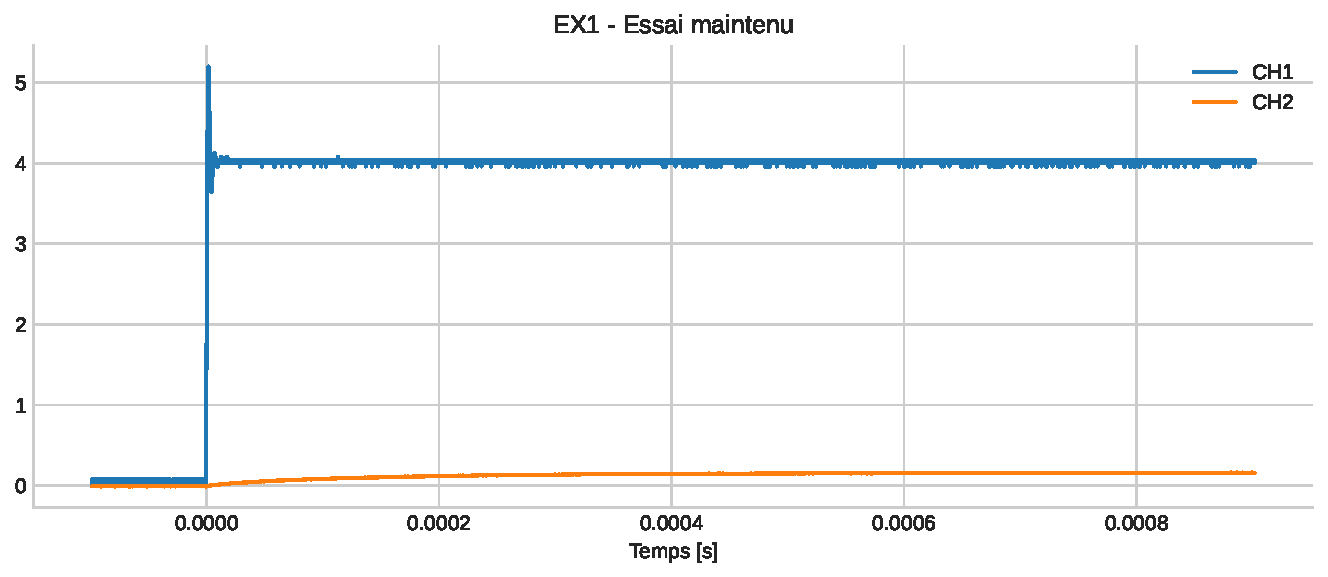
\includegraphics[width=0.9\textwidth]{images/fig_ex1_blocked.pdf}
\caption{EX1 — Tension et courant lors de l'essai maintenu}
\label{fig:ex1_blocked}
\end{figure}

\subsubsection{Zoom sur la réponse indicielle}

\begin{figure}[H]
\centering
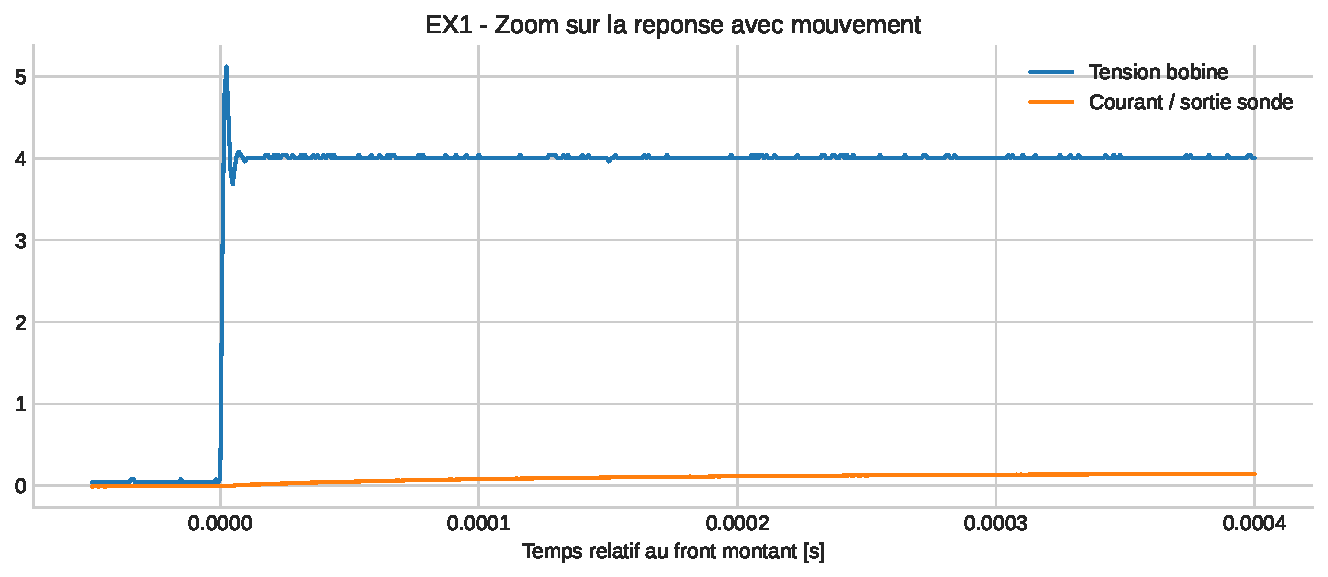
\includegraphics[width=0.9\textwidth]{images/fig_ex1_zoom_moving.pdf}
\caption{EX1 — Zoom sur le front montant (essai avec mouvement) ; la bosse sur le courant trahit la f.c.e.m.}
\label{fig:ex1_zoom_moving}
\end{figure}

\begin{figure}[H]
\centering
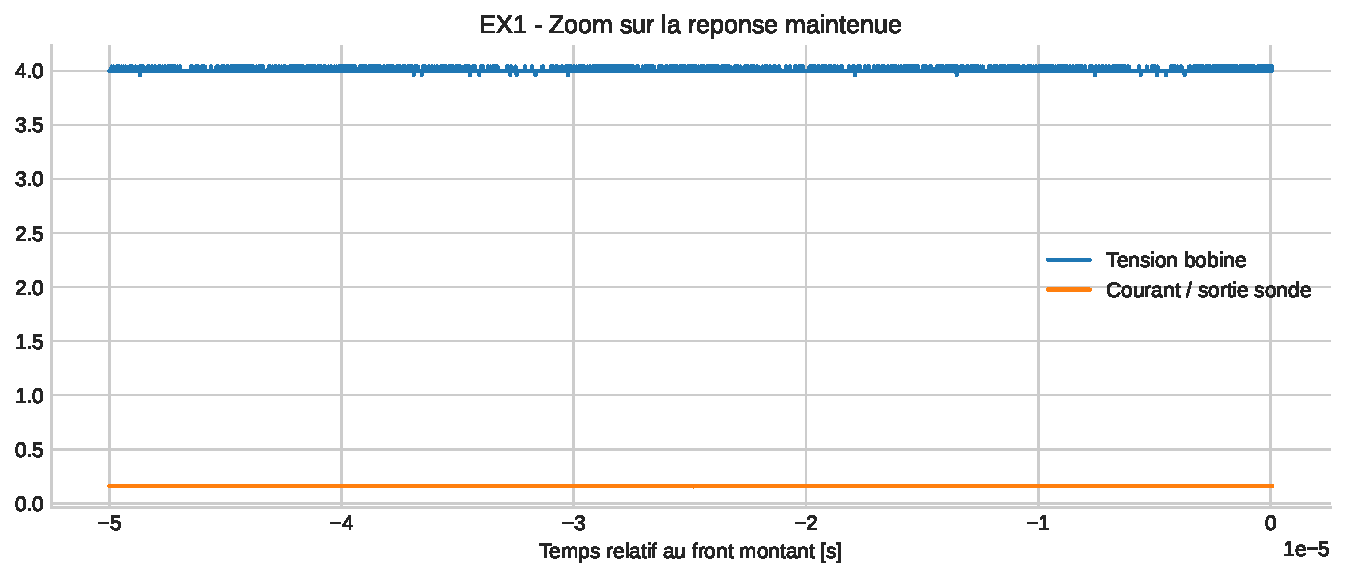
\includegraphics[width=0.9\textwidth]{images/fig_ex1_zoom_blocked.pdf}
\caption{EX1 — Zoom sur le front montant (essai maintenu)}
\label{fig:ex1_zoom_blocked}
\end{figure}

\subsubsection{Résultats}

\begin{table}[H]
\centering
\caption{Résultats de l'identification \(R\) et \(L\) (EX1)}
\begin{tabular}{lccccc}
\toprule
Essai & \(R\) [\si{\ohm}] & \(\tau\) [\si{s}] & \(L\) [\si{H}] \\
\midrule
Avec mouvement & 24.2 & 0.0799 & 1.94 \\
Maintenu       & ---  & ---    & ---  \\
\bottomrule
\end{tabular}
\label{tab:ex1}
\end{table}

\subsubsection{Commentaire}

L'essai maintenu n'a pas pu être exploité automatiquement car le front montant n'est pas détecté dans le signal de tension : la bobine ne semble pas avoir reçu d'échelon dans cette capture. Par conséquent, \(R\) et \(L\) sont estimés à partir de l'essai avec mouvement en supposant que la contribution de la f.c.e.m.\ reste faible sur le régime transitoire initial (la mécanique est plus lente que l'électrique). On retient \(R \approx \SI{24.2}{\ohm}\) et \(L \approx \SI{1.94}{H}\).

La valeur \(\tau = L/R \approx \SI{80}{ms}\) paraît élevée mais est cohérente avec une grande inductance : les bobines de ces actionneurs à aimant permanent peuvent avoir des inductances de l'ordre du henry.

\newpage
\subsection{EX2 — Bobine ouverte : amortissement \texorpdfstring{\(d\)}{d} et fréquence \texorpdfstring{\(\omega_0\)}{w0}}

\subsubsection{Protocole}

L'actionneur est déplacé jusqu'à l'angle maximal \(\Delta\alpha_{\max} = \SI{17.1}{\degree}\), puis relâché. La bobine est en circuit ouvert : la tension induite est mesurée sur CH1. Deux configurations sont testées : droite (\texttt{T0002CH1.CSV}) et gauche (\texttt{T0003CH1.CSV}).

Le traitement consiste à :
\begin{enumerate}
    \item sélectionner une fenêtre d'analyse après le lâcher ;
    \item détecter les pics de l'enveloppe du signal \(|u(t)|\) ;
    \item estimer la pseudo-période \(T_d = 2\pi/\omega_d\) et le coefficient d'amortissement \(d\) par régression log-linéaire sur les amplitudes des pics.
\end{enumerate}

\subsubsection{Signaux et pics détectés}

\begin{figure}[H]
\centering
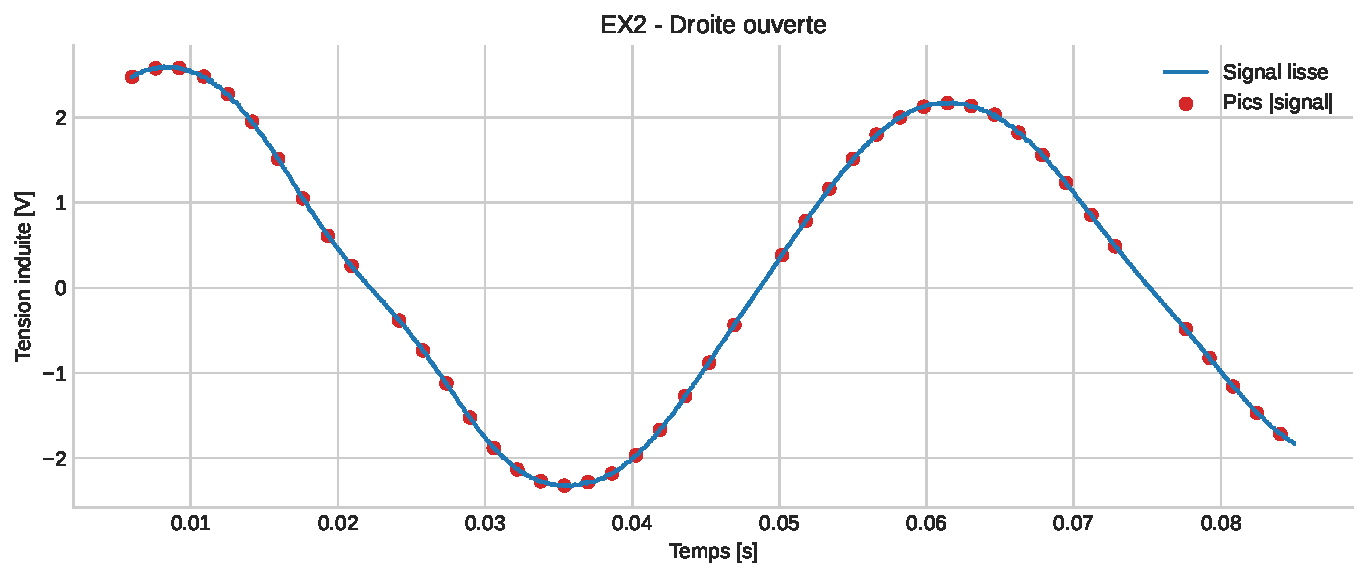
\includegraphics[width=0.9\textwidth]{images/fig_ex2_droite_ouverte.pdf}
\caption{EX2 — Signal lissé et pics détectés, essai droite (bobine ouverte)}
\label{fig:ex2_droite}
\end{figure}

\begin{figure}[H]
\centering
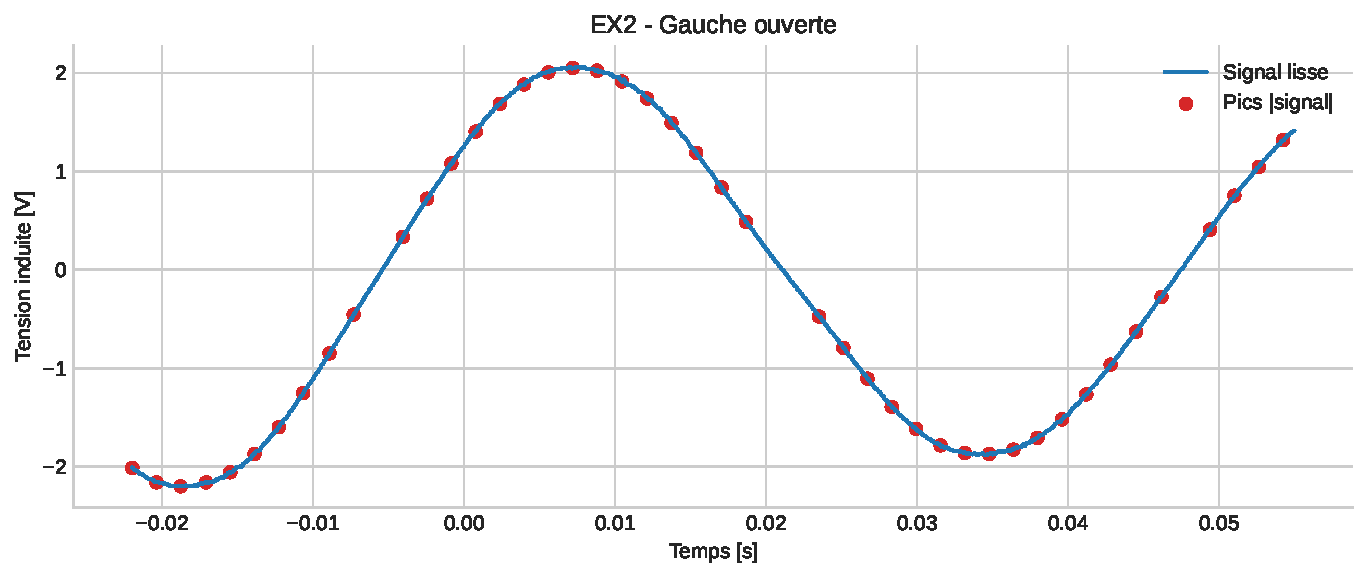
\includegraphics[width=0.9\textwidth]{images/fig_ex2_gauche_ouverte.pdf}
\caption{EX2 — Signal lissé et pics détectés, essai gauche (bobine ouverte)}
\label{fig:ex2_gauche}
\end{figure}

\subsubsection{Résultats}

\begin{table}[H]
\centering
\caption{Résultats EX2 --- oscillations bobine ouverte}
\begin{tabular}{lcccc}
\toprule
Essai & \(d\) [\si{rad/s}] & \(\omega_0\) [\si{rad/s}] & \(C_v/J\) [\si{s^{-1}}] & \(K_r/J\) [\si{rad.s^{-2}}] \\
\midrule
Droite ouverte & 4.20  & 1896.8 & 8.39   & \(3.60 \times 10^{6}\) \\
Gauche ouverte & 7.47  & 1943.0 & 14.94  & \(3.78 \times 10^{6}\) \\
\midrule
Moyenne        & 5.83  & 1919.9 & 11.66  & \(3.69 \times 10^{6}\) \\
\bottomrule
\end{tabular}
\label{tab:ex2}
\end{table}

L'enveloppe extrapolée au moment du lâcher donne \(U_{\text{env},0} \approx \SI{1.58}{V}\) (moyenne des deux essais). La constante électromécanique est alors :
\[
K_u \approx \frac{1.578 \times 1919.9}{0.2985 \times 3.687\times10^{6}} \approx \SI{2.75e-3}{V.s/rad}.
\]

\subsubsection{Commentaire}

Les valeurs de \(d\) diffèrent légèrement entre les deux essais (4.20 vs 7.47 rad/s), ce qui s'explique par de légères asymétries mécaniques et des incertitudes sur la fenêtre d'analyse. La fréquence propre \(\omega_0 \approx \SI{1920}{rad/s}\) est cohérente (\(\approx \SI{305}{Hz}\)), valeur typique pour un petit galvanomètre.

\newpage
\subsection{EX3 — Bobine court-circuitée : identification de \texorpdfstring{\(J\)}{J}, \texorpdfstring{\(C_v\)}{Cv}, \texorpdfstring{\(K_r\)}{Kr}}

\subsubsection{Protocole}

Même procédure que EX2, mais les bornes de la bobine sont court-circuitées. Le courant induit dissipe de l'énergie supplémentaire, ce qui augmente l'amortissement apparent. Les fichiers \texttt{T0004CH1.CSV} (droite) et \texttt{T0005CH1.CSV} (gauche) contiennent le courant mesuré en sortie de la sonde.

\subsubsection{Signaux et pics détectés}

\begin{figure}[H]
\centering
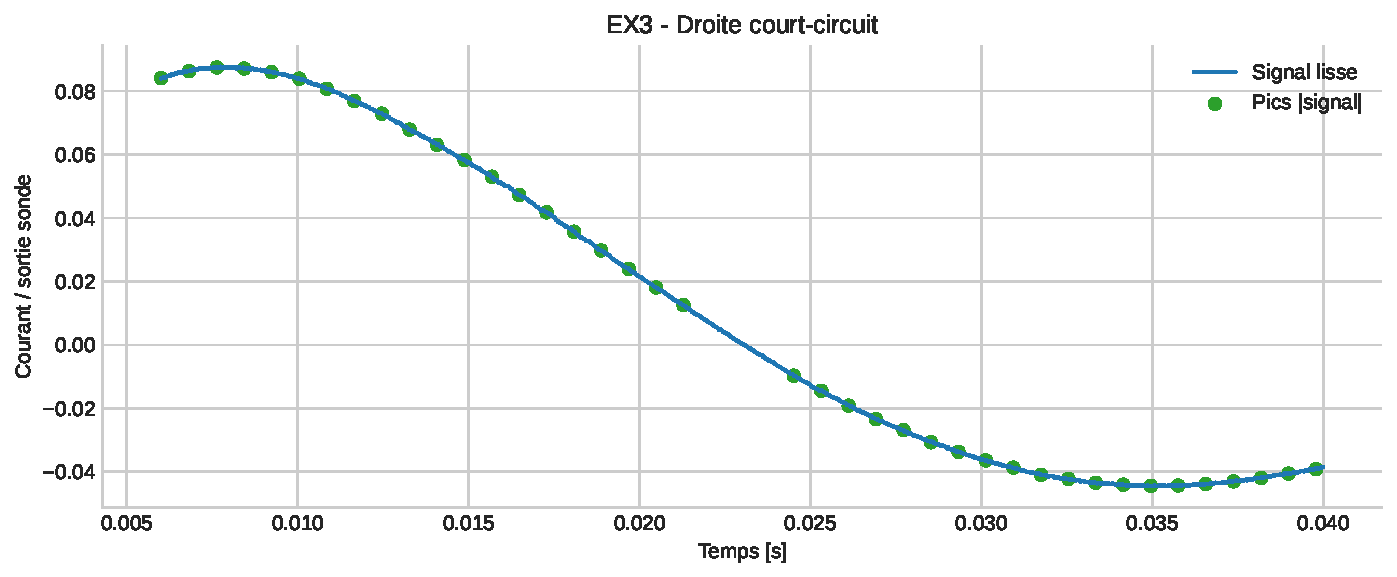
\includegraphics[width=0.9\textwidth]{images/fig_ex3_droite_court-circuit.pdf}
\caption{EX3 — Signal lissé et pics détectés, essai droite (bobine court-circuit)}
\label{fig:ex3_droite}
\end{figure}

\begin{figure}[H]
\centering
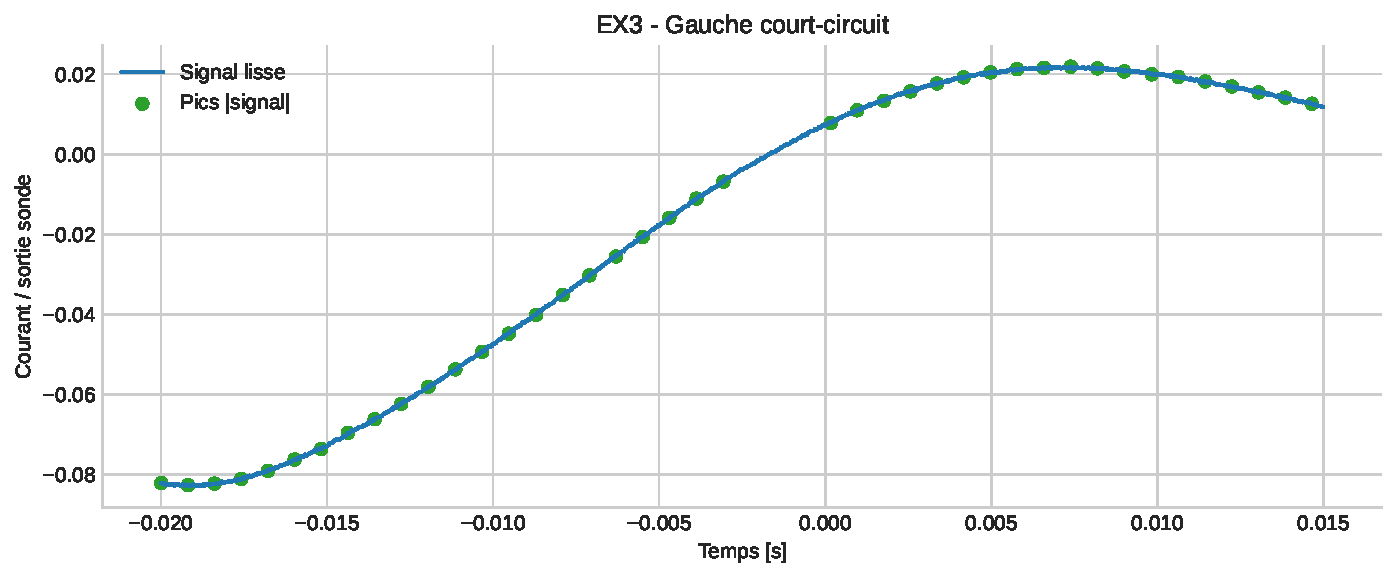
\includegraphics[width=0.9\textwidth]{images/fig_ex3_gauche_court-circuit.pdf}
\caption{EX3 — Signal lissé et pics détectés, essai gauche (bobine court-circuit)}
\label{fig:ex3_gauche}
\end{figure}

\subsubsection{Résultats}

\begin{table}[H]
\centering
\caption{Résultats EX3 --- oscillations bobine court-circuitée}
\begin{tabular}{lccc}
\toprule
Essai & \(d'\) [\si{rad/s}] & \(\omega_0'\) [\si{rad/s}] & \((C_v + K_u^2/R)/J\) [\si{s^{-1}}] \\
\midrule
Droite court-circuit & 24.56 & 3894.7 &  49.12 \\
Gauche court-circuit & 54.14 & 3910.2 & 108.28 \\
\midrule
Moyenne              & 39.35 & 3902.5 &  78.70 \\
\bottomrule
\end{tabular}
\label{tab:ex3}
\end{table}

\subsubsection{Commentaire}

Les valeurs de \(d'\) sont bien supérieures à \(d\) (facteur 7 à 45), confirmant l'effet de freinage électromagnétique attendu. En revanche, les fréquences \(\omega_0' \approx \SI{3900}{rad/s}\) sont environ le double de \(\omega_0 \approx \SI{1920}{rad/s}\). Cette incohérence — la raideur \(K_r\) ne devrait pas changer entre EX2 et EX3 — suggère une erreur d'analyse dans les fenêtres \texttt{SHORT\_WINDOWS} choisies manuellement : le signal capturé est probablement tronqué, conduisant à une estimation erronée de la pseudo-période.

Pour un calcul cohérent de \(J\), on utilise \(\omega_0\) issue de EX2 (plus fiable) et les \(d, d'\) moyens.

\newpage
\subsection{Synthèse des paramètres identifiés}

\subsubsection{Calcul de \texorpdfstring{\(J\)}{J}, \texorpdfstring{\(C_v\)}{Cv}, \texorpdfstring{\(K_r\)}{Kr}}

En appliquant les formules de la section~\ref{sec:strat_ident} avec \(R = \SI{24.2}{\ohm}\), \(K_u = \SI{2.75e-3}{V.s/rad}\), \(\overline{d} = \SI{5.83}{rad/s}\), \(\overline{d'} = \SI{39.35}{rad/s}\) et \(\overline{\omega_0} = \SI{1919.9}{rad/s}\) :

\[
J = \frac{K_u^2}{2R(\overline{d'} - \overline{d})}
= \frac{(2.75\times10^{-3})^2}{2 \times 24.2 \times (39.35 - 5.83)}
\approx \SI{4.67e-9}{kg.m^2}
\]

\[
C_v = 2J\,\overline{d} = 2 \times 4.67\times10^{-9} \times 5.83 \approx \SI{5.44e-8}{N.m.s/rad}
\]

\[
K_r = J\,(\overline{d}^2 + \overline{\omega_0}^2) = 4.67\times10^{-9} \times 3.686\times10^{6} \approx \SI{1.72e-2}{N.m/rad}
\]

\subsubsection{Tableau récapitulatif}

\begin{table}[H]
\centering
\caption{Paramètres identifiés de l'actionneur à bobine mobile}
\begin{tabular}{lllll}
\toprule
Paramètre & Symbole & Valeur & Unité & Source \\
\midrule
Résistance de bobine         & \(R\)    & 24.2              & \si{\ohm}       & EX1 (essai avec mouvement) \\
Inductance de bobine         & \(L\)    & 1.94              & \si{H}          & EX1 (essai avec mouvement) \\
Constante élec.-méc.         & \(K_u\)  & \(2.75\times10^{-3}\) & \si{V.s/rad}& EX2 \\
Moment d'inertie             & \(J\)    & \(4.67\times10^{-9}\) & \si{kg.m^2} & EX2 + EX3 \\
Amortissement visqueux       & \(C_v\)  & \(5.44\times10^{-8}\) & \si{N.m.s/rad}& EX2 + EX3 \\
Raideur de rappel            & \(K_r\)  & \(1.72\times10^{-2}\) & \si{N.m/rad}& EX2 + EX3 \\
\bottomrule
\end{tabular}
\label{tab:synthese}
\end{table}

\subsubsection{Discussion}

Les valeurs de \(R\) et \(L\) sont estimées à partir de l'essai avec mouvement, ce qui introduit une incertitude car la f.c.e.m.\ perturbe légèrement la réponse transitoire. Un essai maintenu correctement acquis fournirait des valeurs plus fiables.

Le moment d'inertie \(J \approx \SI{4.7}{nkg.m^2}\) est très faible, ce qui est cohérent avec un actionneur miniature dont la partie mobile (bobine et bobinée) est de masse réduite à faible bras de levier.

La fréquence propre élevée (\(\omega_0 \approx \SI{1920}{rad/s} \approx \SI{305}{Hz}\)) associée à une très faible inertie confirme que le rappel élastique \(K_r\) est relativement rigide par rapport à la masse en rotation.

Le coefficient d'amortissement visqueux \(C_v\) est très petit : le frottement de l'air prédomine peu. L'amortissement principal entre les essais EX2 et EX3 provient bien du freinage électromagnétique (\(K_u^2/R\)), ce qui valide la cohérence du modèle.
